% last updated in April 2002 by Antje Endemann
% Based on CVPR 07 and LNCS, with modifications by DAF, AZ and elle, 2008 and AA, 2010, and CC, 2011; TT, 2014; AAS, 2016

\documentclass[runningheads]{llncs}
\usepackage{graphicx}
\usepackage{amsmath,amssymb} % define this before the line numbering.
\usepackage{ruler}
\usepackage{color}
\usepackage{enumitem}
\usepackage[ruled,vlined]{algorithm2e}
\usepackage[width=122mm,left=12mm,paperwidth=146mm,height=193mm,top=12mm,paperheight=217mm]{geometry}
\DeclareMathOperator*{\argmin}{\arg\!\min\,}
\begin{document}
% \renewcommand\thelinenumber{\color[rgb]{0.2,0.5,0.8}\normalfont\sffamily\scriptsize\arabic{linenumber}\color[rgb]{0,0,0}}
% \renewcommand\makeLineNumber {\hss\thelinenumber\ \hspace{6mm} \rlap{\hskip\textwidth\ \hspace{6.5mm}\thelinenumber}}
% \linenumbers
\pagestyle{headings}
\mainmatter
\def\ECCV18SubNumber{***}  % Insert your submission number here

\def\eg{\textit{e.g.}}
\def\etal{\textit{et al.}}

\title{Deep Convolutional Compressed Sensing for LiDAR Depth Completion} % Replace with your title

\titlerunning{ECCV-18 submission ID \ECCV18SubNumber}

\authorrunning{ECCV-18 submission ID \ECCV18SubNumber}

\author{Anonymous ECCV submission}
\institute{Paper ID \ECCV18SubNumber}



\maketitle

\begin{abstract}
The abstract should summarize the contents of the paper. LNCS guidelines
indicate it should be at least 70 and at most 150 words. It should be set in 9-point
font size and should be inset 1.0~cm from the right and left margins.
\dots
\keywords{We would like to encourage you to list your keywords within
the abstract section}
\end{abstract}

% \section{Introduction}
    In recent years 3D information has become an important component of robotic sensing. Usually this information in 2.5D as a depth map, either measured directly using LIDAR or computed using stereo correspondence. Since LIDAR and stereo techniques yield few samples relative to modern image sensors, it has become desirable to convert sparse depth measurements into high resolution depth maps.\\
  The field of compressed sensing (CS) provides a natural framework for this  problem of recovering a signal from only a few measurements. Formally, compressed sensing is concerned with solving the following optimization problem:
  \begin{equation}
    \label{eq:1}
    \min \left||x\right||_0 s.t. Ax = b
  \end{equation}
  The key insight is that when the optimal $x$ is known to have only a few non-zero entries, then it is a unique minimum and can be recovered exactly even when $A$ is over-complete and only a few elements of $b$ are known.\\
  The choice of dictionary, $A$, is extremely important for extracting sparse codes $x$ but learning an appropriate $A$ from data proves challenging, especially with a large amount of data or large dimensionality. Learning dictionaries is especially difficult in layered sparse coding where one seeks a very high level sparse representation $x_{\ell}$ such that $b = A_0A_1\ldots A_{\ell}x_{\ell}$ and each intermediate product $x_i = A_iA_{i+1}\ldots A_{\ell}x_{\ell}$ is also sparse. This formulation makes using large effective dictionary computationally tractable, and when the dictionaries have a convolutional structure it allows for increased receptive fields while keeping the number of parameters manageable. For the case of depth map prediction, dictionary learning is further complicated by the fact that we do not have any complete signals to learn from. Dictionary learning algorithms exist for single-layer sparse training data case, and for the multi-level case, but not for learning multi-level codes from sparse data. This is reflected by the fact that recent work applying CS to depth completion has used single-level, hand crafted dictionaries. In this work we propose an algorithm for learning all dictionaries and codes simultaneously from a large dataset of sparse ground-truth.\\
  Unlike CS, deep learning techniques can be directly applied to sparse inputs, sparse ground truth, and large training sets. However, for deep networks to be effective at dealing with sparse inputs they require orders of magnitude more parameters and data than our method while still not performing as well. Urhig et al pointed out the issues of CNNs with sparse inputs and proposed Sparsity Invariant CNNs which achieve good performance on sparse data with much shallower networks. While these new networks explicitly handle the sparsity of the input, they do not explicitly handle the constraint that the input depth map is a subset of the desired output. The recent work by Payan et al.~\cite{papyan}  shows a connection between deep learning and sparse coding, where feed forward neural networks are viewed as a single iteration of a sparse coding algorithm. With this perspective they introduce Alternating Direction Neural Networks which internally perform the ADMM optimization algorithm. In this work we propose an extension of ADMMs which explicitly encode the previously mentioned sparsity and input/output constraints.\\
  To summarize the three main contributions of this paper are:
  \begin{enumerate}
    \item Our method provides a way to learn all dictionaries directly from the data. CS dictionary learning algorithms exist, but are limited to single level codes and are not applicable to learning from incomplete training data, as is our case. Additionally, recent applications of CS to depth completion have not used any learning and instead rely on hand crafted dictionaries such as wavelets and contourlets.
  \item Our method uses very few parameters compared to deep learning approaches. We achieve state of the art performance using only two layers of convolutional dictionaries which require several orders of magnitude fewer parameters than modern deep networks. With fewer parameters, our system trains faster and with less data.
  \item Our method allows for explicit encoding of the constraints from the input sparse depth. Current deep learning approaches simply feed a sparse depth map into a network and hope that it learns to identify which inputs represent missing data. Some recent models explicitly include masks which drastically improves CNN performance, but none have a way of encoding that the input is a subset of the desired output. In contrast our method directly optimizes the predicted map with respect to the input.
  \end{enumerate}
  
\section{Introduction}
\begin{figure}
\centering
  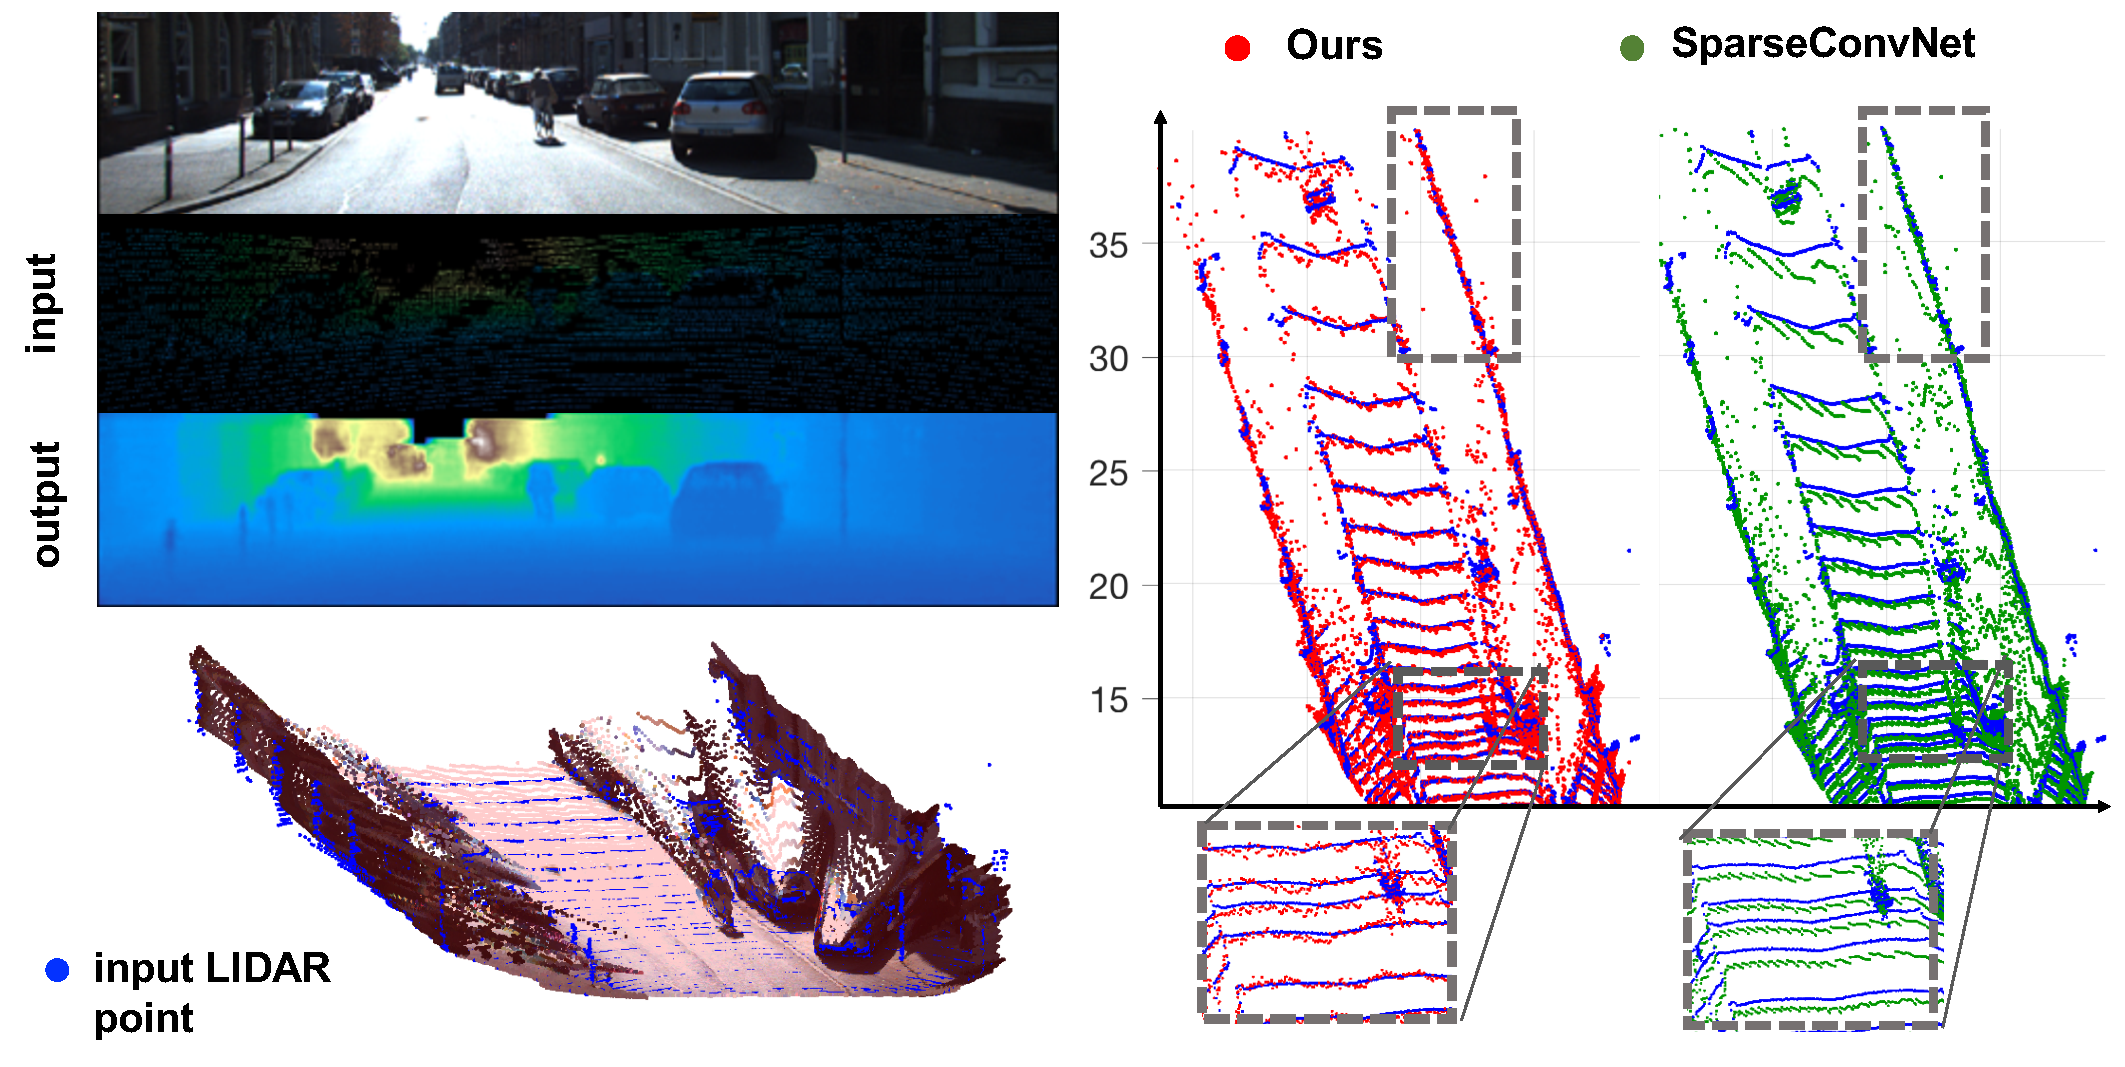
\includegraphics[width=\textwidth]{figs/keyfig.pdf}\\
%   
\includegraphics[width=0.6\textwidth]{intro-ground}\\
%   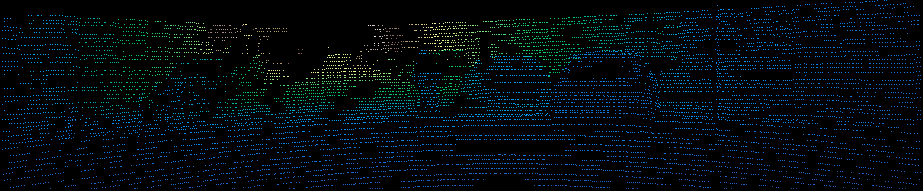
\includegraphics[width=0.6\textwidth]{intro-input}\\
%   
\includegraphics[width=0.6\textwidth]{intro-pred}
  \caption{The bicyclist and bollards can barely be seen in the input map but a clearly represented in the output. Our method also accurately reconstructs very thin objects such as the sign post. On the right it can be seen that our method enforces that its prediction should match the input points while the SparseConvNet systematically underestimates the depth.}
  \label{fig:intro}
\end{figure}
In recent years 3D information has become an important component of robotic sensing. Usually this information is presented in 2.5D as a depth map, either measured directly using LIDAR or computed using stereo correspondence. Since LIDAR and stereo techniques yield few samples relative to modern image sensors, it has become desirable to convert sparse depth measurements into high resolution depth maps as shown in Figure (\ref{fig:intro}).


Recent works~\cite{sparsetodense,uhrig} have directly applied deep networks to depth completion from sparse measures. However, common network architectures have two drawbacks when applied to this task: 1) They implicitly pose depth completion as finding a mapping from sparse depth maps to dense ones, instead of as finding a depth map that is consistent with the sparse input. This essentially throws away information and we observe that feed forward networks do not learn to propagate the input points through to the output. Qualitative evidence of this can be seen in Figure (\ref{fig:intro}). 2) Common networks are sensitive to the sparsity of the input since they treat all pixels equally, regardless of whether or not they represent samples or missing input. Special CNN networks have been designed to address this problem, but they still do not express the constraints given by the input~\cite{uhrig}. In this paper we address both of these issues with a novel deep recurrent autoencoder architecture, which internally optimizes its depth prediction with respect to both sparsity and input constraints.
%) Common networks are sensitive to the sparsity level of the input since they treat each pixel equally, regardless of whether it is an input or missing value. While special CNN architecture have been designed to achieve sparsity invariance~\cite{}, they have no way to handle the second issue. 2) Common networks do not explicitly enforce the constraint that the input depth map is a subset of the desired output. In fact, we observe that deep networks are not able to effectively propagate input depth samples to the output. In this paper we address both of these issues with a novel deep recurrent autoencoder architecture which internally optimizes its depth prediction while respecting to both sparsity and input constraints.
To do this, we have taken inspiration from Compressed sensing (CS) which provides a natural framework for this problem. Formally, CS is concerned with recovering signals from incomplete measurements by enforcing that signals be sparse when measured in an appropriate basis. This basis takes the form of an overcomplete matrix which maps sparse representations to observed signals.
% To reconstruct signals which are not measured, certain prior knowledge/assumption of the signal is required.

The choice of dictionary is crucial for recovering the signal efficiently, especially when the dimensionality is high. For high resolution imagery data, such as depth maps, multi-layer convolutional sparse coding (CSC)~\cite{papyan} is effective as it explicitly models local interactions through the convolution operator with tractable computational and model complexity. However, none of the existing multi-layer convolutional sparse coding algorithms are designed for learning from sparse ground truth data. This is reflected by the fact that recent works~\cite{hawe2011dense,liu2015depth} applying CS to depth completion are restricted to using single-level, hand crafted dictionaries. CS has also fallen out of fashion since the existing algorithms have difficult to interpret hyper-parameters, and often do not achieve good performance without careful tuning of these parameters.

% extracting sparse codes $x$ but learning an appropriate $A$ from data proves challenging, especially with a large amount of data or large dimensionality. Learning dictionaries is especially difficult in layered sparse coding where one seeks a very high level sparse representation $x_{\ell}$ such that $b = A_0A_1\ldots A_{\ell}x_{\ell}$ and each intermediate product $x_i = A_iA_{i+1}\ldots A_{\ell}x_{\ell}$ is also sparse. This formulation makes using large effective dictionary computationally tractable, and when the dictionaries have a convolutional structure it allows for increased receptive fields while keeping the number of parameters manageable. For the case of depth map prediction, dictionary learning is further complicated by the fact that we do not have any complete signals to learn from. 
% Dictionary learning algorithms exist for single-layer sparse training data case, and for the multi-level case, but not for learning multi-level codes from sparse data. 

Recent developments in the formal analysis of deep learning have shown that convolutional neural networks and convolutional sparse coding are closely related. Specifically it has been shown that CNNs with Relu activation functions are carrying out a specific form of the layered thresholding algorithm for CSC. Layered thresholding is a simple algorithm for solving multi-layered convolutional sparse coding problems which can be effective when there is little noise and the coherence of the dictionary is high. Motivated by the work of Murdock \etal, in this paper we propose a network architecture which encodes a more sophisticated algorithm for ML-CSC. Encoding the ML-CSC objective in a deep network allows us to learn the dictionaries and parameters together in an end to end fashion. We show that by better approximating this objective, we can out perform all published results on the KITTI depth completion benchmark while using far fewer parameters and layers. Furthermore, this work builds on the Alternating Direction Neural Network (ADNN) framework of Murdock \etal which gives theoretical insight into deep learning and we believe is a promising new area of research.

%Following the recent work of Murdock \etal, which shows that feed forward neural networks can be viewed as a single iteration of alternating direction method of multipliers (ADMM) for sparse coding, we unroll the ADMM optimization iterations for CS and express it as a deep recurrent autoencoder. This not only allows us to learn multi-layer dictionaries and hyper-parameters, in an end-to-end fashion, but also gives a concrete framework for explicitly enforcing constraints on the output of a network.

% propose an extension of ADNNs which explicitly encode the previously mentioned sparsity and input/output constraints.


% On the other hand, recent works~\cite{} have directly applied deep networks to depth completion from sparse measures. However, common network architectures applied to this task have two drawbacks: 1) Common networks are sensitive to the sparsity level of the input as they treats each pixel equally, whether it's an input or missing value. While special CNN architecture were designed to achieve sparsity invariance~\cite{}, our method is free from this issue by the nature of CS; 2) Common networks do not explicitly enforce the constraint that the input depth map is a subset of the desired output. In fact, we observe cases where network gives wrong prediction at pixels where ground truth is already given as input. In comparison, our approach directly optimize the prediction to minimize the reconstruction error of the input.



% Urhig et al~\cite{} proposed Sparsity Invariant CNNs which achieve good performance on sparse data with much shallower networks. 
% However, for deep networks to be effective at dealing with sparse inputs they require orders of magnitude more parameters and data than our method while still not performing as well. Urhig et al pointed out the issues of CNNs with sparse inputs and proposed Sparsity Invariant CNNs which achieve good performance on sparse data with much shallower networks. While these new networks explicitly handle the sparsity of the input, they do not explicitly enforce the constraint that the input depth map is a subset of the desired output. 
% With this perspective they introduce Alternating Direction Neural Networks which internally perform the ADMM optimization algorithm. \\

To summarize, the main contributions of this paper are:
\begin{enumerate}
\item We frame an end-to-end multi-layer dictionary learning algorithm as a neural network. This allows us to effectively learn dictionaries and hyper-parameters from a large dataset. In comparison, existing CS algorithms either use hand crafted dictionaries, separately learned multi-level dictionaries, or are inapplicable to incomplete training data~\cite{sulam}, as is our case.

  
\item Our method allows for explicit encoding of the constraints from the input sparse depth. Current deep learning approaches~\cite{sparsetodense} simply feed in a sparse depth map and rely solely on data to teach the network to identify which inputs represent missing data. Some recent models~\cite{uhrig} explicitly include masks to achieve sparsity invariant, but none have a guaranteed way of encoding that the input is a subset of the desired output. In contrast our method directly optimizes the predicted map with respect to the input.
  
  
\item Our method demonstrates state-of-the-art performance with much fewer parameters compared to deep networks. In fact, using only two layers of dictionaries and 1600 parameters, our method already substantially outperforms modern deep networks which use more than 20 layers and over 3 million parameters~\cite{sparsetodense}. As a result of having fewer parameters, our approach trains faster and requires less data.
  
\end{enumerate}
  
\section{Method}
\section{Experiments}

\subsection{Implementation Details}
\label{sec:impl-deta}

We implemented three variants of algorithm (\ref{alg:dcsc}) for the cases $\ell = 1,2,3$. For the single layer case we let $W^T_1$ be a 11x11 convolution with striding of 2 and 8 filters. For $\ell = 2$ we let $W^T_{1}$ be an 11x11 convolution with 8 filters and $W^T_{1}$ be a 7x7 convolution with 16 filters. Finally for the $\ell = 3$ case: $W^T_{1}$ is an 11x11 convolution with 8 filters, $W^T_{2}$ is a 7x7 convolution with 16 filters, and $W^T_{3}$ is a 5x5 convolution with 32 filters. For both $\ell = 2$ and $\ell = 3$, all convolutions have striding of 2. For the single layer case we learned the dictionaries with the number of iterations set to 5 and then at test time increased the number of iterations to 20. For the two and three layer cases the number of iterations was fixed at train and test time to 10 except in section \ref{sec:effect-iter-optim} where the number of test and training iterations is varied. All training was done with the ADAM optimizer with the default parameters.
\subsection{KITTI Depth Completion Benchmark}
\label{sec:kitti-depth-compl}
\begin{figure}
\begin{tabular}{r|cc}
  \label{table:kitti}
  & RMSE (m) & MAE (m)\\\hline
  Bilateral NN~\cite{} & 4.19 & 1.09\\
  SGDU~\cite{} & 2.5 & 0.72\\
  Fast Bilateral Solver~\cite{} & 1.98 & 0.65\\
  TGVL~\cite{} & 4.85 & 0.59\\\hline
  Closest Depth Pooling & 2.77 & 0.94\\
  Nadaraya Watson~\cite{} & 2.99 & 0.74\\
  ConvNet & 2.97 & 0.78\\
  ConvNet + mask & 2.24 & 0.79\\
  SparseConvNet~\cite{} & 1.82 & 0.58\\
  Ma \& Karaman & 1.68 & 0.70\\\hline
  Ours 1 Layer & 2.77 & 0.83\\
  Ours 2 Layers & 1.44 & 0.47\\
  Ours 3 Layers & \textbf{1.37} & \textbf{0.46}
\end{tabular}

\caption{Validation error of various methods on the KITTI Depth Completion benchmark. All resulsts except for SparseConvNet and Ma's are taken as reported from ~\cite{}. Our method outperforms all previous state-of-the-art depth only completion methods (Middle) as well as those that use RGB images for guidance (Top).}
\label{fig:kitti}
\end{figure}

The KITTI dataset provides raw LIDAR measurements in conjunction with high resolution RGB images from 22 video sequences of driving in both cities and highways. Combining all video sequences gives 93k frames with semi-dense ground truth depth. However, these measurements are corrupted by noise, motion of the vehicle during sampling, and image rectification artifacts. Additionally the raw LIDAR points are very sparse, accounting for only 4\% of the total number of pixels in the map. For these reasons the raw KITTI dataset is not ideal for evaluating depth completion systems.\\

The sparsity issue can be resolved by accumulating LIDAR measurements from nearby frames in the video sequences, and by using semi-global matching to reconstruct dense 3D points which can be projected using the given calibration files. Both these processes introduce more errors from occlusion and non-rigid movement across frames. Urhig \etal resolved these issues by automatically removing accumulated LIDAR points that deviate too far from the SGM points. The result is the KITTI depth completion benchmark, the first and only large scale dataset for depth completion training and evaluation. This benchmark is ideal since it has high quality ground truth and effectively simulates the main application of depth completion: recovering dense depth from a single LiDAR sweep.\\

Urhig \etal then evaluated their proposed Sparsity Invariant CNNs on this dataset as well as several other current methods for depth completion. Figure (\ref{fig:kitti}) shows the results they present along with our method and the results of the very deep Sparse-to-Dense network proposed by Ma \& Karaman. The Sparse-to-Dense network is fairly standard, using Resnet-18 as an encoder and up-projection blocks for a decoder. Similar architectures have been presented in other works for single shot depth prediction. Notably our method outperforms all of the existing methods by a wide margin, including those that use RGB images and those that use orders of magnitude more parameters than our method.
\subsection{Effect of Amount of Training Data}
\label{sec:effect-training-data}
\begin{figure}
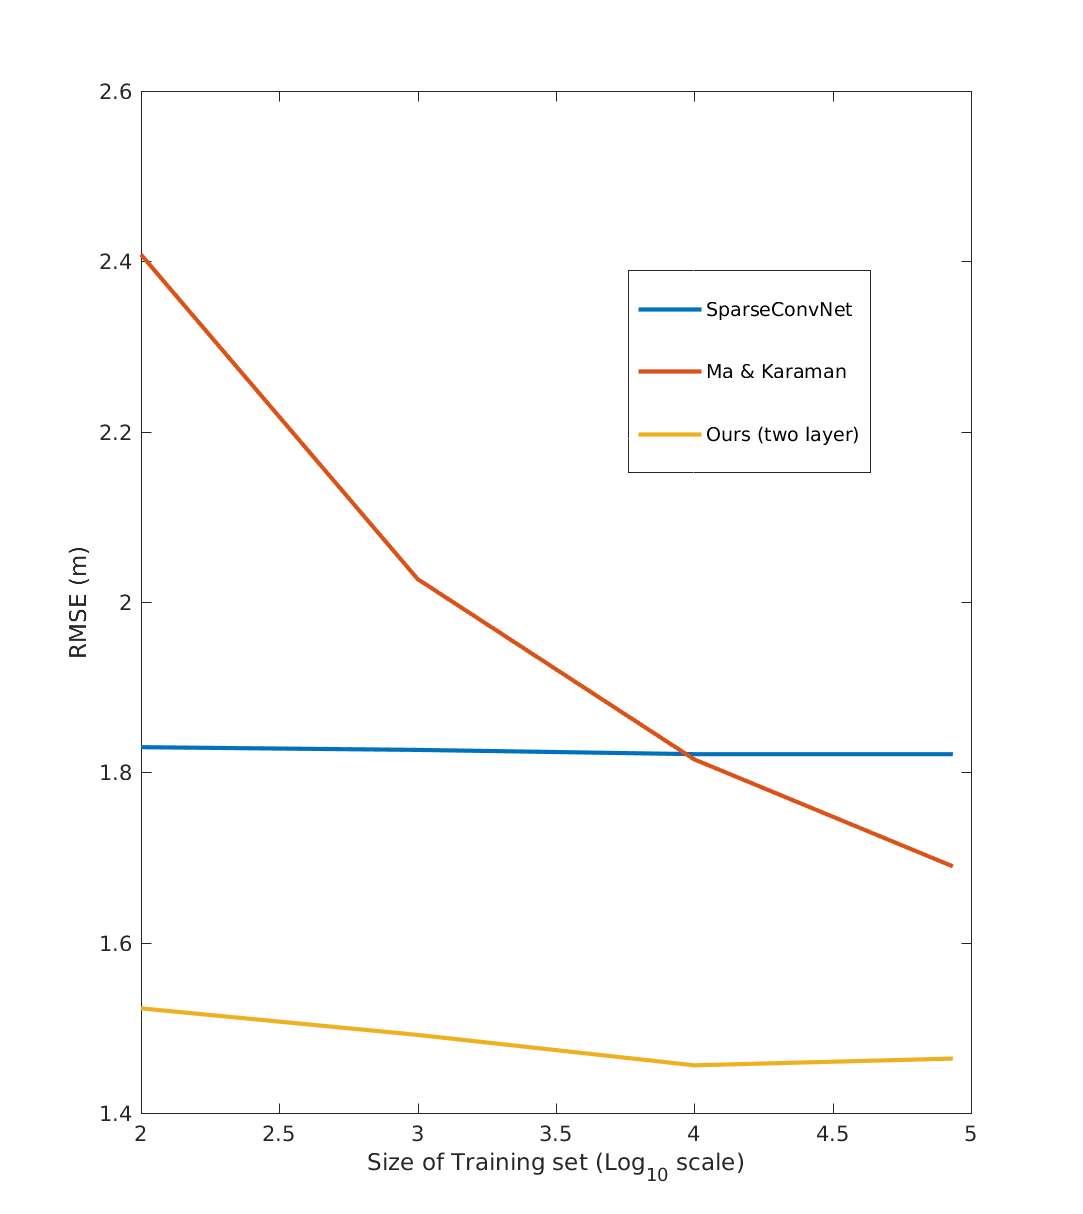
\includegraphics[width=0.45\textwidth]{trainsizeplot}
  \caption{Results of selected methods for varying training set sizes.}
  \label{fig:trainsize}
\end{figure}
Modern deep learning models typically have tens of thousands to millions of parameters and therefore require enormous training sets to achieve good performance. This is in fact the motivation for the KITTI depth completion dataset, since previous benchmarks did not have enough data to train deep networks. In this section we investigate the dependence on the amount of training data on the performance of our method in comparison with a standard deep network and the sparsity invariant variety.\\
Figure (\ref{fig:trainsize}) shows the results of evaluating these models on the 1k manually selected validation depth maps after training on varying subsets of the 86k training maps. Our method outperforms both baselines for all training sizes. As expected Ma \& Karaman's method fails to generalize well when trained on a small dataset since the model has ~3.4M parameters but performs well once trained on the full dataset. It is interesting to observe that the method of Urhig \etal does not gain any performance from training on more data. Our method is able to perform comparably to the sparsity invariant network with only 100 training examples but does increase in performance when given more data, validating the need for learning layered sparse coding dictionaries from large training sets.
\subsection{Effect of Iterative Optimization}
\label{sec:effect-iter-optim}
\begin{figure}
  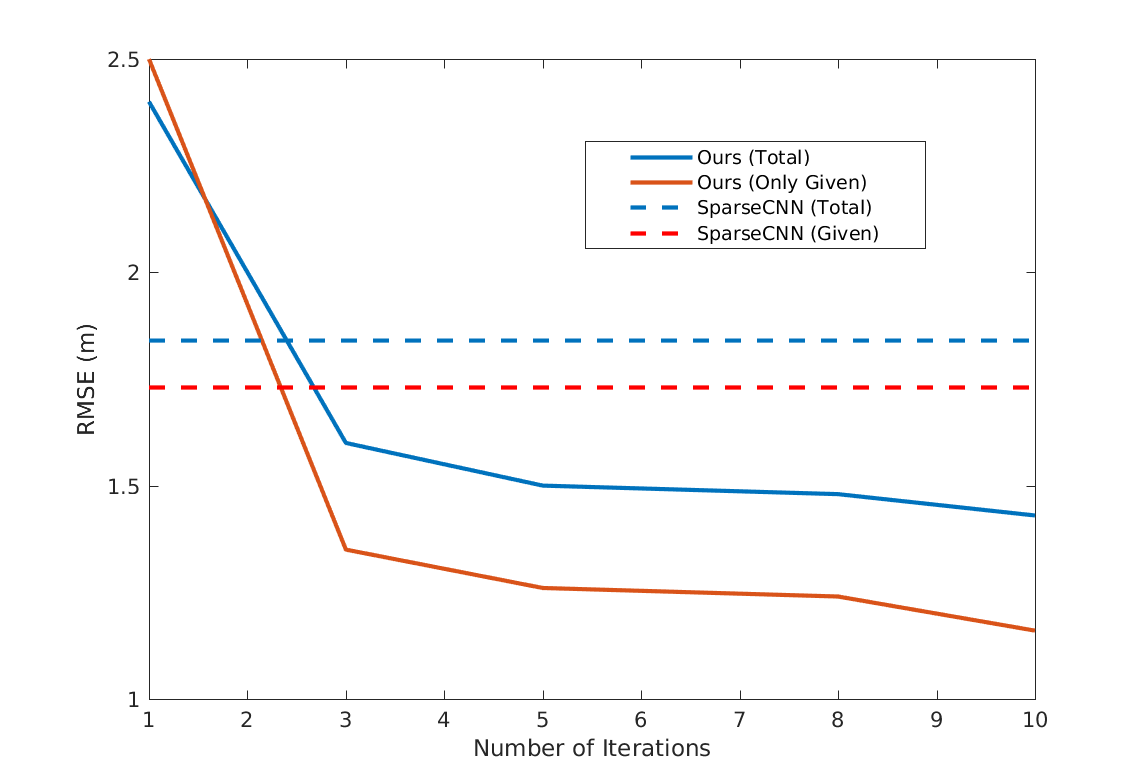
\includegraphics[width=0.45\textwidth]{iterplot}
  \caption{Results on the depth completion benchmark for different numbers of ADMM iterations. The total error is shown in blue while the red line shows the error on just those points given as input. The dotted lines show the same metrics but for the SparseConvNet of Urhig \etal}
  \label{fig:iterplot}
\end{figure}

In this section we demonstrate that the success of our approach comes from its ability to refine depth estimates over multiple iterations. Applying a feed forward neural network to this problem frames it as finding a mapping from sparse LiDAR points to true depth maps. This is a reasonable approach but it doesn't utilize all of the available information, specifically it doesn't encode the relationship that input samples are a subset of the output. In contrast, our approach of phrasing depth completion as a compressed sensing missing data problem directly expresses that relationship. By solving this problem in an iterative fashion our network that is able to find depth maps that are both consistent with the input constraints and have sparse representations.\\

The importance iterative optimization is shown in Figure (\ref{fig:iterplot}) where we examine the performance of our method as a function of the number of ADMM iterations it uses. It is clear that with few iterations our network fails to enforce the constraints and performs comparably to the SparseConvNet. As we increase the number of iterations that our method can meet the constraints and greatly out perform existing methods.
% - Feed-forward is bad for this problem
% - Phrasing it as optimization is better, specifically sparse coding
% - All the best algorithms for CSC require multiple iterations to converge to a good solution
% - We have evidence for this, more iteration decreases both the total error and the error on the constraint points

% - instead of viewing problem as mapping from sparse input to dense depth we define it as an optimization problem over the given depth values and their sparse codes.
% - 




\end{document}